\documentclass[english, aspectratio=169]{beamer}
% english is for the language used in standard texts (figures, tables etc)
% aspectratio of 16:9 or set it for more old school to 4:3 (without the ':')

% ---------------------------------------------------------------------------- %
% Load base preamble
% ---------------------------------------------------------------------------- %
\usepackage{import}
\subimport{./preamble/}{beamer.tex}

% ---------------------------------------------------------------------------- %
% Local settings
% ---------------------------------------------------------------------------- %
\newcommand{\B}[0]{\ensuremath{\mathbb{B}}}

\newcommand{\sort}[1]{\text{sort}(#1)}

\newcommand{\triple}[3]{\ensuremath{(#1, #2, #3)}}
\renewcommand{\arc}[3]{\ensuremath{#1 \xrightarrow{_{#2}} #3}}

% colors
\newcommand{\tikzdot}[1]{
  \protect\tikz[baseline=-3.4pt]{
    \fill[color=#1, opacity=0.7] circle[radius=1.7pt];
  }
}

\tikzstyle{dots_significant}=[only marks, mark=o, mark size=1.8pt, mark options={color=black, opacity=0.9}]

\colorlet{qbf}{cyan}
\tikzstyle{dots_qbf}=[only marks, mark=*, mark size=1.8pt, mark options={color=qbf, fill=qbf, opacity=0.5}]
\tikzstyle{x_qbf}=[only marks, mark=x, mark size=2.2pt, mark options={color=qbf, fill=qbf, opacity=0.7}]
\tikzstyle{plot_qbf}=[color=qbf, dashed, line width=0.7pt, opacity=0.7]

\colorlet{goe}{orange}
\tikzstyle{dots_goe}=[only marks, mark=*, mark size=1.8pt, mark options={color=goe, fill=goe, opacity=0.5}]
\tikzstyle{x_goe}=[only marks, mark=x, mark size=2.2pt, mark options={color=goe, fill=goe, opacity=0.7}]
\tikzstyle{plot_goe}=[color=goe, dashed, line width=0.7pt, opacity=0.7]

% ------------------------------------------------------------------------------
%
% ------------------------------------------------------------------------------
% Opener:
% - ???
%
% Key points:
% - Apply-Reduce (TACAS 22)
%   - Example Animation (single variable quantification)
%   - Does not scale well for multiple variables...
% - Nested Apply-Reduce (TACAS 25)
%   - Example Animation
%   - Theoretical Results
%   - Experimental Results
%
% Take Home Message:
% - ???

% ------------------------------------------------------------------------------
% TITLEPAGE
% ------------------------------------------------------------------------------
\title{Multi-variable Quantification of BDDs\\in External Memory using Nested Sweeping}

\author{\textbf{Steffan Christ S\o lvsten}, Jaco van de Pol}

\institute{
\includegraphics[width=0.2\linewidth]{external/aulogo_uk_var2_black.eps}}

\date{TACAS 2025}

\begin{document}
\titleframe

\begin{frame}[plain,noframenumbering]
  % Let's go back to 1986, the year of the:
  % - Last time Halley's comet flew by (2nd of January)
  % - Chernobyl disaster (26th of April)
  % - Start of the "Kartoffelkur" (13th of October)

  \begin{center}
    \bf
    {\fontsize{42}{50}\selectfont \faIcon{backward}}

    \vspace{10pt}

    {\Huge 1986}
  \end{center}
\end{frame}


\begin{frame}
  \frametitle{Binary Decision Diagrams}

  \begin{columns}
    \begin{column}{0.4\linewidth}
      \begin{figure}
        \centering

        \begin{subfigure}{1\linewidth}
          \centering

          \begin{tikzpicture}[scale=0.9, every node/.style={transform shape}]
              % nodes
  \node[shape = circle, draw = black]
  (0) {$x_0$};

  \node[shape = circle, draw = black, below right= .4cm and .5cm of 0]
  (1) {$x_1$};

  \node[shape = circle, draw = black, below left=.4cm and .5cm of 1]
  (2) {$x_2$};

  \node[shape = circle, draw = black, below left=.4cm and .5cm of 2]
  (31) {$x_3$};
  \node[shape = circle, draw = black, below right=.4cm and .5cm of 2]
  (32) {$x_3$};

  % leafs
  \node[shape = rectangle, draw = black, below=.4cm of 31]
  (sink_T) {$\top$};

  \node[shape = rectangle, draw = black, below=.4cm of 32]
  (sink_F) {$\bot$};

  % arcs
  \draw[->, dashed]
    (0)  edge (2)
    (1)  edge (2)
    (2)  edge (31)
    (31) edge (sink_T)
    (32) edge (sink_F)
  ;

  \draw[->]
    (0)  edge (1)
    (1)  edge (32)
    (2)  edge (32)
    (31) edge (sink_F)
    (32) edge (sink_T)
  ;
          \end{tikzpicture}

          \caption{$(x_0 \wedge x_1 \wedge x_3) \vee (x_2 \oplus x_3)$}
        \end{subfigure}
      \end{figure}
    \end{column}
    \begin{column}{0.59\linewidth}
      \only<2>{
        \begin{theorem}[Bryant~'86]
          Given a fixed variable order, a (Reduced Ordered) Binary Decision Diagram is a unique
          canonical representation of a Boolean function.
        \end{theorem}
      }

      \only<4->{
        \begin{theorem}[Bryant~'86]
          Given BDDs $\phi$ and $\psi$, $\phi \odot \psi$ is computible in
          $\Oh{\abs{\phi} \cdot \abs{\psi}}$ time.
        \end{theorem}

        \medskip

        \begin{theorem}[Bryant~'86]
          Given BDD $\phi$ and Boolean $b$, $\phi[x_i \mapsto b]$ is computible in
          $\Oh{\abs{\phi}}$ time.
        \end{theorem}

        \medskip

        \begin{corollary}
          Given BDD $\phi$, $\exists x_i .\ \phi(x)$ requires $\Oh{\abs{\phi}^2}$
          time.
        \end{corollary}
        \vspace{-5pt}
        \begin{proof}
          $\exists x_i . \phi(x_i) \equiv \phi[x_i \mapsto \bot] \lor \phi[x_i \mapsto \top]$
        \end{proof}
      }
    \end{column}
  \end{columns}
\end{frame}

\begin{frame}[plain,noframenumbering]
  % Let's go somewhat forwards in time to 1996, where:
  % - Dolly the cloned sheep is born (5th of July)
  % - Charles and Diana get a dirvoce (28th of August)
  % - Copenhagen is "European Capital of Culture" of the year

  \begin{center}
    \bf
    {\fontsize{42}{50}\selectfont \faIcon{forward}}

    \vspace{10pt}

    {\Huge 1996}
  \end{center}
\end{frame}

\iffalse
\begin{frame}[fragile]
  \frametitle{$\exists x_i.\ \phi(x_i)$}

  \begin{figure}
    \centering

    \begin{lstlisting}
  *@{\bf exists}@*($f$, $x_i$)
      if $f = \bot \lor f = \top$
          return $f$
      if $f$.var = $x_i$
          return *@{\bf or}@*($f$.low, $f$.high)
      else
          exi0 := *@{\bf exists}@*($f$.low, $X$)
          exi1 := *@{\bf exists}@*($f$.high, $X$)
          return Node { $f$.var, exi0, exi1 }
    \end{lstlisting}
    \caption{A recursive single-variable {\bf exists} operation.}
  \end{figure}
\end{frame}
\fi

\begin{frame}
  \frametitle{$\exists x_i .\ \phi(x_i)$}

  \begin{figure}
    % tikz/tandem.tex (but simplified)

    \centering
    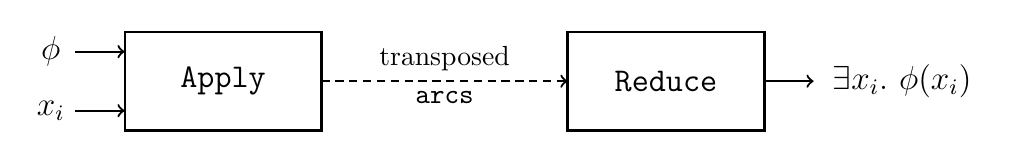
\begin{tikzpicture}[scale=1.25]
      % Boxes
      \draw[color=black, thick]
        (0,0) rectangle ++(2,1)
        node[pos=.5]{\large \texttt{Apply}}
      ;
      \draw[color=black, thick]
        (4.5,0) rectangle ++(2,1)
        node[pos=.5]{\large \texttt{Reduce}}
      ;

      % Arcs
      \draw[->, color=black, thick]
        (-0.5,0.8) -- ++(0.5,0)
        node[pos=-0.5]{\large $\phi$}
      ;
      \draw[->, color=black, thick]
        (-0.5,0.2) -- ++(0.5,0)
        node[pos=-0.5]{\large $x_i$}
      ;

      \draw[densely dashed, ->, thick] (2,0.5) -- ++(2.5,0)
        node[pos=0.5,above]
        {transposed}
        node[pos=0.5,below]
        {\texttt{arcs}}
      ;

      \draw[->, color=black, thick]
        (6.5,0.5) -- ++(0.5,0)
        node[pos=2.8]{\large $\exists x_i.\ \phi(x_i)$}
      ;
    \end{tikzpicture}
  \end{figure}
\end{frame}

\begin{frame}
  \frametitle{$\exists x_i .\ \phi(x_i)$ : \texttt{Apply}}

  \begin{center}
  \begin{tikzpicture}
    % Sweepline
    \onslide<2> { \draw[gray, thick, dashed] (-3, 0) -- (10, 0); }
    \onslide<3> { \draw[gray, thick, dashed] (-3, -0.9) -- (10, -0.9); }
    \onslide<4> { \draw[gray, thick, dashed] (-3, -1.85) -- (10, -1.85); }
    \onslide<5> { \draw[gray, thick, dashed] (-3, -2.9) -- (10, -2.9); }
    \onslide<6> { \draw[gray, thick, dashed] (-3, -3.9) -- (10, -3.9); }
    \onslide<7> { \draw[gray, thick, dashed] (-3, -4.75) -- (10, -4.75); }

    % INPUT
    \draw[black, thick] (0.1,0.1)  -- (1.8,-1.85)  -- (1.5,-3.9)  -- (0.81,-5.7)
                        (-0.1,0.1) -- (-1.8,-1.8) -- (-1.5,-3.9) -- (-0.8,-5.7);

    \node[shape = circle, draw = black, fill = white]
    (i_root) {};

    \onslide<2-> {
      \node[shape = circle, draw = black, fill = white,
            below right=0.65cm and 0.1cm of i_root]
      (i_p1) {};

      \draw[->] (i_root) edge (i_p1);
    }

    \onslide<3-> {
      \node[shape = circle, draw = black, fill = white,
            below left=0.65cm and 0.1cm of i_p1]
      (i_p2) {};

      \draw[->, dashed] (i_p1) edge (i_p2);
    }

    \onslide<4-> {
      \node[shape = circle, draw = black, fill = white,
            below right=0.7cm and 0.1cm of i_p2]
      (i_quant) {\tiny $x_i$};

      \draw[->] (i_p2) edge (i_quant);
    }

    \onslide<5-> {
      \node[shape = circle, draw = black, fill = white,
            below left =0.65cm and 0.1cm of i_quant]
      (i_p3_1) {};

      \node[shape = circle, draw = black, fill = white,
            below right =0.65cm and 0.1cm of i_quant]
      (i_p3_2) {};

      \draw[->, dashed] (i_quant) edge (i_p3_1);

      \draw[->] (i_quant) edge (i_p3_2);
    }

    \onslide<6-> {
      \node[shape = circle, draw = black, fill = white,
            below left =0.6cm and 0.2cm of i_p3_1]
      (i_p4_1) {};

      \draw[->, dashed] (i_p3_1) edge (i_p4_1);

      \node[shape = circle, draw = black, fill = white,
            below left =0.6cm and 0.2cm of i_p3_2]
      (i_p4_2) {};

      \draw[->, dashed] (i_p3_2) edge (i_p4_2);
    }

    \onslide<7-> {
      \node[shape = rectangle, draw = black, fill = white,
            below left=5.4cm and 0.2cm of i_root]
      (i_p5_1) {};

      \node[shape = rectangle, draw = black, fill = white,
            below right=5.4cm and 0.2cm of i_root]
      (i_p5_2) {};

      \draw[->] (i_p4_1) edge (i_p5_1);
      \draw[->] (i_p4_2) edge (i_p5_2);
    }

    % OUTPUT
    \onslide<3-> {
      \draw[black, densely dotted, thick]
        (6.5,0.1)  -- (7.4,-0.9)
        (6.25,0.1) -- (5.35,-0.9)
      ;

      \node[shape = circle, draw = black, fill = white,
            right=6cm of i_root]
      (o_root) {};

      \node[shape = circle, draw = black, fill = white,
            below right=0.65cm and 0.1cm of o_root]
      (o_p1) {};

      \draw[->, black] (o_p1) edge (o_root);
    }

    \onslide<4-> {
      \draw[black, densely dotted, thick]
        (7.4,-0.9)  -- (8.2,-1.85)
        (5.35,-0.9) -- (4.55,-1.85)
      ;

      \node[shape = circle, draw = black, fill = white,
            below left=0.65cm and 0.1cm of o_p1]
      (o_p2) {};

      \draw[->, black, dashed] (o_p2) edge (o_p1);
    }

    \onslide<5> {
      \draw[black, dotted, thick]
        (8.2,-1.85) -- (8.45, -2.9)
        (4.55,-1.85) -- (4.27,-2.9)
      ;
    }

    \onslide<6-> {
      \draw[black, densely dotted, thick]
        (8.2,-1.85) -- (8.7, -3.9)
        (4.55,-1.85) -- (4,-3.9)
      ;

      \node[shape = circle, draw = black, fill = white,
            below right=1.78cm and 0.1cm of o_p2]
       (o_p3) {};

       \draw[->, black] (o_p3) edge (o_p2);
    }

    \onslide<7-8> {
      \draw[black, densely dotted, thick]
        (8.7, -3.9) -- (8.6, -4.75)
        (4,-3.9) -- (4.2,-4.75)
      ;

      \node[shape = circle, draw = black, fill = white,
            below left =0.6cm and 0.1cm of o_p3]
      (o_p4) {};

      \draw[->, black, dashed] (o_p4) edge (o_p3);

      \node[shape = rectangle, draw = black, fill = white,
            below =5.4cm of o_root]
      (o_p5) {};

      \draw[->, black] (o_p5) edge (o_p4);

      \draw[black, densely dotted, thick] (8.6, -4.75) -- (8,-5.7)
      (4.2,-4.75)  -- (4.8,-5.7);
    }
  \end{tikzpicture}
\end{center}
\end{frame}

\begin{frame}
  \frametitle{$\exists x_i .\ \phi(x_i)$ : \texttt{Reduce}}

  \begin{center}
  \begin{tikzpicture}
    % Sweepline
    \onslide<2> { \draw[gray, thick, dashed] (-1, -4.75) -- (12, -4.75); }
    \onslide<3> { \draw[gray, thick, dashed] (-1, -3.9)  -- (12, -3.9); }
    \onslide<4> { \draw[gray, thick, dashed] (-1, -1.85) -- (12, -1.85); }
    \onslide<5> { \draw[gray, thick, dashed] (-1, -0.9)  -- (12, -0.9); }
    \onslide<6> { \draw[gray, thick, dashed] (-1, 0)     -- (12, 0); }

    % INPUT
    \draw[black, densely dotted, thick]
      % left-hand side
         (0.8,-5.7) -- (0.2,-4.75) -- (0.0,-3.9) --  (0.55,-1.85) -- (1.35,-0.9) -- (2.25,0.1)
      % right-hand side
      -- (2.5,0.1)  -- (3.4,-0.9) -- (4.2,-1.85) -- (4.7, -3.9) -- (4.6, -4.75) -- (4,-5.7)
    ;

    \onslide<5->{
      \node[shape = circle, draw = black, fill = white] at (2.4, 0.0)
      (i_root) {};
    }

    \onslide<4->{
      \node[shape = circle, draw = black, fill = white,
            below right=0.65cm and 0.1cm of i_root]
      (i_p1) {};
    }
    \onslide<5->{
      \draw[->, black] (i_p1) edge (i_root);
    }

    \onslide<3->{
      \node[shape = circle, draw = black, fill = white,
            below left=0.65cm and 0.1cm of i_p1]
      (i_p2) {};
    }
    \onslide<4->{
      \draw[->, black, dashed] (i_p2) edge (i_p1);
    }

    \onslide<2->{
      \node[shape = circle, draw = black, fill = white,
            below right=1.78cm and 0.1cm of i_p2]
       (i_p3) {};
    }
    \onslide<3->{
      \draw[->, black] (i_p3) edge (i_p2);
    }

    \onslide<2->{
      \node[shape = circle, draw = black, fill = white,
            below left =0.6cm and 0.1cm of i_p3]
      (i_p4) {};

      \draw[->, black, dashed] (i_p4) edge (i_p3);

      \node[shape = rectangle, draw = black, fill = white,
            below =5.4cm of i_root]
      (i_p5) {};

      \draw[->, black] (i_p5) edge (i_p4);
    }

    % OUTPUT
    \onslide<2->{
      \draw[black, thick]
        % left-hand side
        (7.4,-4.75) -- (7.8,-5.7)
        % right-hand side
        (9.9, -4.75) -- (9.4,-5.7)
      ;

      \node[shape = rectangle, draw = black, fill = white,
            right =6cm of i_p5]
      (o_p5) {};

      \node[shape = circle, draw = black, fill = white,
            above =0.6cm of o_p5]
      (o_p4) {};

      \draw[->, black] (o_p5) edge (o_p4);
    }

    \onslide<3->{
      \draw[black, thick]
        % left-hand side
        (7.3,-3.9) -- (7.4,-4.75)
        % right-hand side
        (10.0, -3.9) -- (9.9, -4.75)
      ;

      \node[shape = circle, draw = black, fill = white,
            above right=0.6cm and 0.1cm of o_p4]
      (o_p3) {};

      \draw[->, black, dashed] (o_p4) edge (o_p3);
    }

    \onslide<4->{
        \draw[black, thick]
        % left-hand side
        (7.4,-1.85) -- (7.3,-3.9)
        % right-hand side
        (9.9,-1.85) -- (10.0, -3.9)
      ;

      \node[shape = circle, draw = black, fill = white,
            above left=1.8cm and 0.1cm of o_p3]
      (o_p2) {};

      \draw[->, black] (o_p3) edge (o_p2);
    }

    \onslide<5->{
      \draw[black, thick]
        % left-hand side
        (7.75,-0.9) -- (7.4,-1.85)
        % right-hand side
        (9.5,-0.9) -- (9.9,-1.85)
      ;

      \node[shape = circle, draw = black, fill = white,
            above right=0.68cm and 0.1cm of o_p2]
      (o_p1) {};

      \draw[->, black, dashed] (o_p2) edge (o_p1);
    }

    \onslide<6->{
      \draw[black, thick]
        % left-hand side
        (8.65,0.1) -- (7.75,-0.9)
        % right-hand side
        (8.9,0.1)  -- (9.5,-0.9)
      ;

      \node[shape = circle, draw = black, fill = white,
            right =6cm of i_root]
      (o_root) {};

      \draw[->, black] (o_p1) edge (o_root);
    }
  \end{tikzpicture}
\end{center}
\end{frame}

\begin{frame}
  \frametitle{$\exists x_i .\ \phi(x_i)$}

  \begin{theorem}[Lars Arge~'96]
    Given BDDs $\phi$ and $\psi$, $\phi \odot \psi$ is computible in
    $\Oh{\sort{\abs{\phi} \cdot \abs{\psi}}}$ time and I/Os.
  \end{theorem}

  \medskip

  \begin{theorem}[S{\o}lvsten et al.~'22]
    Given BDD $\phi$ and Boolean $b$, $\phi[x_i \mapsto b]$ is computible in
    $\Oh{\sort{\abs{\phi}}}$ time and I/Os.
  \end{theorem}

  \medskip\pause

  \begin{corollary}[S{\o}lvsten et al.~'22]
    Given BDD $\phi$, the time and I/O complexity of quantification is
    \vspace{-8pt}
    \begin{itemize}
    \item $\Oh{\sort{\abs{\phi}^2}}$ for a single variable.
    \item $\Oh{\sort{\abs{\phi}^{2^k}}}$ for $k$ variables.
    \end{itemize}
  \end{corollary}
\end{frame}

\begin{frame}[plain,noframenumbering]
  % Let's go to the recent year of 2022, where:
  % - A picture is taken of the Sagittarius A* black hole (12th of May)
  % - Russia invades Ukraine (24th of February)
  % - Denmark lifts all restrictions due to the COVID-19 pandemic (1st of February)

  \begin{center}
    \bf
    {\fontsize{42}{50}\selectfont \faIcon{forward}}

    \vspace{10pt}

    {\Huge 2022}
  \end{center}
\end{frame}

\begin{frame}%[plain,noframenumbering]{} % \blankframe until reveal
  \begin{center}
    {\fontsize{42}{50}\selectfont \textbf{Adiar}}

    \textcolor{gray}{\large \em
      I/O-efficient Decision Diagrams
    }

    \vspace{-10pt}
    \rule{180pt}{0.6pt}
    \vspace{-5pt}

    \textcolor{gray}{\small
      \href{http://github.com/ssoelvsten/adiar}{github.com/ssoelvsten/adiar}
    }
  \end{center}
\end{frame}

\begin{frame}[plain,noframenumbering]
  % Let's go to the present day, where:
  % - ???

  \begin{center}
    \bf
    {\fontsize{42}{50}\selectfont \faIcon{forward}}

    \vspace{10pt}

    {\Huge 2025}
  \end{center}
\end{frame}

\iffalse
\begin{frame}[fragile]
  \frametitle{$\exists \vec{x}.\ \phi(\vec{x})$}

  \begin{figure}
    \centering

    \begin{lstlisting}
  *@{\bf exists}@*($f$, $X$)
      if $f = \bot \lor f = \top$
          return $f$
      exi0 := *@{\bf exists}@*($f$.low, $X$)
      exi1 := *@{\bf exists}@*($f$.high, $X$)
      if $f$.var $\in$ $X$
          return *@{\bf or}@*(exi0, exi1)
      else
          return Node { $f$.var, exi0, exi1 }
    \end{lstlisting}
    \caption{A (nested) recursive multi-variable {\bf exists} operation.}
  \end{figure}
\end{frame}
\fi

\begin{frame}
  \frametitle{$\exists \vec{x}.\ \phi(\vec{x})$}

  \begin{figure}
    \centering
    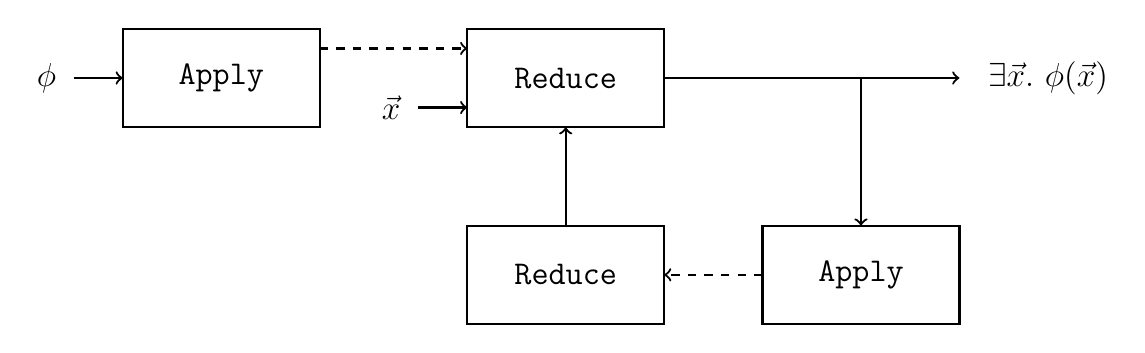
\begin{tikzpicture}[scale=1.25]
      % Boxes (outer)
      \draw[thick] (0,0) rectangle ++(2,1)
      node[pos=.5]{\large \texttt{Apply}};
      \draw[thick] (3.5,0) rectangle ++(2,1)
      node[pos=.5]{\large \texttt{Reduce}};

      % Arcs (outer)
      \draw[->, thick] (-0.5,0.5) -- ++(0.5,0)
      node[pos=-0.55]{\large $\phi$};

      \draw[->, thick, dashed] (2,0.8) -- ++(1.5,0);

      \draw[->, thick] ( 3.0,0.2) -- ++(0.5,0)
      node[pos=-0.55]{\large $\vec{x}$};

      \draw[->, thick] (5.5,0.5) -- ++(3,0)
      node[pos=1.3]{\large $\exists \vec{x}.\ \phi(\vec{x})$};

      % Boxes (inner)
      \draw[thick] (6.5,-2) rectangle ++(2,1)
      node[pos=.5]{\large \texttt{Apply}};
      \draw[thick] (3.5,-2) rectangle ++(2,1)
      node[pos=.5]{\large \texttt{Reduce}};

      % Arcs (inner)
      \draw[->, thick] (7.5,0.5) -- ++(0,-1.5);

      \draw[->, thick, dashed] (6.5,-1.5) -- ++(-1.0,0);

      \draw[->, thick] (4.5,-1) -- ++(0,1);
    \end{tikzpicture}
  \end{figure}
\end{frame}

\begin{frame}
  \frametitle{$\exists \vec{x}.\ \phi(\vec{x})$}

  \begin{center}
  \begin{tikzpicture}
    % Sweepline
    \onslide<2> { \draw[gray, thick, dashed] (-2.5, -5.0) -- (10, -5.0); }
    \onslide<3> { \draw[gray, thick, dashed] (-2.5, -4.2) -- (10, -4.2); }
    \onslide<4-9> { \draw[gray, thick, dashed] (-2.5, -3.2) -- (10, -3.2); }

    \onslide<4>   { \draw[gray, thick, dashed] (2.5, -3.4) -- (9.7, -3.4); }
    \onslide<5,9> { \draw[gray, thick, dashed] (2.5, -4.2) -- (9.7, -4.2); }
    \onslide<6-8> { \draw[gray, thick, dashed] (2.5, -5.0) -- (9.7, -5.0); }

    \onslide<10> { \draw[gray, thick, dashed] (-2.5, -2.5) -- (10, -2.5); }
    \onslide<11> { \draw[gray, thick, dashed] (-2.5, -1.7) -- (10, -1.7); }
    \onslide<12> { \draw[gray, thick, dashed] (-2.5, 0) -- (10, 0); }

    % --------------------------------------------------------------------------
    % INPUT
    \draw[black, densely dotted, thick]
      % left-hand side
      (-1.6,-5.6) -- (-1.8,-5.0) -- (-2.0,-4.2) -- (-1.4,-1.7) -- (-0.1,0.1)
      % right-hand side
      -- (0.1,0.1) -- (1.4,-1.7)  -- (2.0,-4.2)  -- (1.8,-5.0) -- (1.6,-5.6);

    \onslide<11-> {
      \node[shape = circle, draw = black, fill = white]
      (i_root) {};
    }

    \onslide<10-> {
      \node[shape = circle, draw = black, fill = white,
            below right=1.4cm and 0.2cm of i_root]
      (i_p1) {};
    }

    \onslide<11-> {
      \draw[->, black] (i_p1) edge (i_root);
    }

    \onslide<3-> {
      \node[shape = circle, draw = black, fill = white,
            below left=0.55cm and 0.2cm of i_p1]
      (i_p2) {};
    }

    \onslide<10-> {
      \draw[->, black, dashed] (i_p2) edge (i_p1);
    }

    \onslide<3-> {
      \node[shape = circle, draw = black, fill = white,
            below right=0.5cm and 0.2cm of i_p2]
      (i_quant2) {\tiny $x_j$};
    }

    \onslide<4-> {
      \draw[->, black, thick] (i_quant2) edge (i_p2);
    }

    \onslide<2-> {
      \node[shape = circle, draw = black, fill = white,
            below left=0.55cm and 0.2cm of i_quant2]
      (i_p3_1) {};

      \node[shape = circle, draw = black, fill = white,
            below right=0.55cm and 0.2cm of i_quant2]
      (i_p3_2) {};
    }

    \onslide<3-> {
      \draw[->, black, thick, dashed] (i_p3_1) edge (i_p2);
      \draw[->, black, dashed] (i_p3_1) edge (i_quant2);
      \draw[->, black] (i_p3_2) edge (i_quant2);
    }

    \onslide<2-> {
      \node[shape = circle, draw = black, fill = white,
            below left=0.55cm and 0.2cm of i_p3_1]
      (i_p4_1) {};

      \node[shape = circle, draw = black, fill = white,
            below left=0.55cm and 0.2cm of i_p3_2]
      (i_p4_2) {};

      \draw[->, black, dashed]
        (i_p4_1) edge (i_p3_1)
        (i_p4_2) edge (i_p3_2)
      ;
    }

    \onslide<2-> {
      \node[shape = rectangle, draw = black, fill = white,
            below right=5.4cm and -0.3cm of i_root]
      (i_p5_1) {};

      \node[shape = rectangle, draw = black, fill = white,
            below right=5.4cm and 0.7cm of i_root]
      (i_p5_2) {};

      \draw[->, black]
        (i_p5_1) edge (i_p4_1)
        (i_p5_2) edge (i_p4_2)
      ;
    }

    % --------------------------------------------------------------------------
    % REDUCED OUTPUT
    \onslide<2-6,8-> {
      \draw[thick] (3.0,-5.0) -- (3.2,-5.6)
                   (5.3,-5.0) -- (5.1,-5.6)
      ;

      \node[shape = rectangle, draw = black, fill = white,
            right=3.5cm of i_p5_1]
      (o1_p5_1) {};

      \node[shape = rectangle, draw = black, fill = white,
            right=3.5cm of i_p5_2]
      (o1_p5_2) {};

      \node[shape = circle, draw = black, fill = white,
            right=3.5cm of i_p4_1]
      (o1_p4_1) {};

      \node[shape = circle, draw = black, fill = white,
            right=3.5cm of i_p4_2]
      (o1_p4_2) {};

      \draw[->]
        (o1_p4_1) edge (o1_p5_1)
        (o1_p4_2) edge (o1_p5_2)
      ;
    }

    \onslide<3-5,9-> {
      \draw[thick] (2.9,-4.2) -- (3.0,-5.0)
                   (5.5,-4.2) -- (5.3,-5.0)
      ;

      \node[shape = circle, draw = black, fill = white,
            right=3.5cm of i_p3_1]
      (o1_p3_1) {};

      \node[shape = circle, draw = black, fill = white,
            right=3.5cm of i_p3_2]
      (o1_p3_2) {};

      \draw[->, dashed]
        (o1_p3_1) edge (o1_p4_1)
        (o1_p3_2) edge (o1_p4_2)
      ;
    }

    \onslide<4> {
      \draw[thick, dotted] (3.2,-3.4) -- (2.9,-4.2)
                           (5.1,-3.4) -- (5.5,-4.2)
      ;
    }

    \onslide<10-> {
      \draw[thick] (2.8,-2.5) -- (2.9,-4.2)
                   (4.8,-2.5) -- (5.5,-4.2)
      ;

      \node[shape = circle, draw = black, fill = white,
            right=3.5cm of i_p2]
      (o1_p2) {};

      \draw[->, dashed] (o1_p2) edge (o1_p3_1);
      \draw[->] (o1_p2) edge (o1_p3_2);
    }

    \onslide<11-> {
      \draw[thick] (2.9,-1.7) -- (2.8,-2.5)
                   (4.6,-1.7) -- (4.8,-2.5)
      ;

      \node[shape = circle, draw = black, fill = white,
            right=3.5cm of i_p1]
      (o1_p1) {};

      \draw[->, dashed] (o1_p1) edge (o1_p2);
    }

    \onslide<12-13> {
      \draw[thick] (3.8,0) -- (2.9,-1.7)
                   (4.0,0) -- (4.6,-1.7)
      ;

      \node[shape = circle, draw = black, fill = white,
            right=3.5cm of i_root]
      (o1_root) {};

      \draw[->] (o1_root) edge (o1_p1);
    }

    % --------------------------------------------------------------------------
    % SECOND SWEEP
    \onslide<5-9> {
      \draw[black, dotted, thick] (6.95, -2.9) -- (6.9,-3.2)
                                  (9.15, -2.9) -- (9.2,-3.2)
          ;

      \draw[black, densely dotted, thick] (6.9,-3.2) -- (6.8, -4.2)
                                          (9.2,-3.2) -- (9.4, -4.2)
      ;

      \node[shape = circle, draw = none, % dummy for crossing in-going arcs
            right=3.5cm of o1_p2]
      (o2_p2) {};

      \node[shape = circle, draw = black, fill = white,
            right=3.5cm of o1_p3_1]
      (o2_p3_1) {};

      \node[shape = circle, draw = black, fill = white,
            right=3.5cm of o1_p3_2]
      (o2_p3_2) {};

      \draw[->, black, dotted, thick] (o2_p3_1) edge (o2_p2);
      \draw[->, black, densely dotted, thick] (o2_p3_2) edge (o2_p2);
    }

    \onslide<6-8> {
      \draw[black, densely dotted, thick] (6.8, -4.2) -- (6.9, -5.0)
                                          (9.4, -4.2) -- (9.3, -5.0)
      ;

      \node[shape = circle, draw = black, fill = white,
            right=3.5cm of o1_p4_1]
      (o2_p4_1) {};

      \node[shape = circle, draw = black, fill = white,
            right=3.5cm of o1_p4_2]
      (o2_p4_2) {};

      \draw[->, black, dashed]
        (o2_p4_1) edge (o2_p3_1)
        (o2_p4_2) edge (o2_p3_2)
      ;

      \draw[black, densely dotted, thick] (6.9, -5.0) -- (7.2, -5.6)
                                          (9.3, -5.0) -- (9.0, -5.6)
      ;

      \node[shape = rectangle, draw = black, fill = white,
            right=3.5cm of o1_p5_1]
      (o2_p5_1) {};

      \node[shape = rectangle, draw = black, fill = white,
            right=3.5cm of o1_p5_2]
      (o2_p5_2) {};

      \draw[->, black]
        (o2_p5_1) edge (o2_p4_1)
        (o2_p5_2) edge (o2_p4_2)
      ;
    }
  \end{tikzpicture}
\end{center}
\end{frame}

\begin{frame}
  \frametitle{$\exists \vec{x}.\ \phi(\vec{x})$}

  \Large

  {\bf Theorem~(S{\o}lvsten et al.~'25)}

  Given BDD $\phi$, the quantification of $k$ variables, $\exists \vec{x}.\ \phi(\vec{x})$,\\
  is computible in $\Oh{\sort{\abs{\phi}^{2^k}}}$ time and I/Os.
\end{frame}

\begin{frame}
  \frametitle{Benchmarks}

  \fcolorbox{goe}{goe!50!white}{%
    \begin{minipage}{1.0\linewidth}
      \begin{block}{Garden-of-Eden}
        Given dimensions $N_1, N_2 \in \N$, determine whether there exists in Conway's \emph{Game of
          Life} an initial state of size $N_1 \times N_2$ that is a \emph{Garden of Eden}, i.e.\ is
        otherwise unreachable.
      \end{block}
    \end{minipage}
  }

  \medskip

  \fcolorbox{qbf}{qbf!50!white}{%
    \begin{minipage}{1.0\linewidth}
      \begin{block}{Quantified Boolean Formula}
        Determine whether a Boolean formula
        $\exists \vec{x_1} \forall \vec{x_2} \dots \exists \vec{x_k} .\ \phi(\vec{x_1}, \vec{x_2},
        \dots, \vec{x_k})$ (or any order of quantifiers) evaluates to $\top$ or $\bot$. For inputs,
        we use the two-player games from:

        Irfansha Shaik and Jaco van de Pol: ``\emph{Concise QBF encodings for games on a grid
          (extended version)}''. arXiv (2023).
      \end{block}
    \end{minipage}
  }
\end{frame}

\begin{frame}
  \frametitle{Benchmarks : Single vs. Nested Quantification}

  \begin{figure}
    \centering

    \begin{tikzpicture}
      \begin{axis}[%
        width=0.92\linewidth, height=0.45\linewidth,
        every tick label/.append style={font=\scriptsize},
        % x-axis
        xlabel={\scriptsize Running Time of Adiar with Single-variable Quantification (s)},
        xmin=0.01,
        xtick={0.01,0.1,1,10,100,1000,10000,100000},
        xmax=100000,
        xmode=log,
        % y-axis
        ylabel={\scriptsize Speed-up with Nested Sweeping},
        ymin=0.125,
        ymax=2,
        ymode=log,
        ytick={0.125, 0.25, 0.5, 1, 2},
        yticklabels={
          $8 \times$,
          $4 \times$,
          $2 \times$,
          $1 \times$,
          $\tfrac{1}{2} \times$
        },
        y dir=reverse,
        % grid
        grid style={dashed,black!12},
        ]

        % 1x line
        \addplot[domain=0.01:1000000, samples=8, color=black]
        {1};

        % average
        \addplot[domain=0.01:1000000, samples=8, style=plot_goe]
        {0.5873};
        \addplot[domain=0.01:1000000, samples=8, style=plot_qbf]
        {0.5848};

        % data
        \addplot+ [forget plot, style=dots_goe]
        table {./data/goe.singleton_vs_nested.tex};
        \addplot+ [forget plot, style=dots_qbf]
        table {./data/qbf.singleton_vs_nested.tex};
      \end{axis}
    \end{tikzpicture}

    {
      \tikzdot{goe} GoE \quad \tikzdot{qbf} QBF
    }

    % \caption{Relative time ($T_{\text{old}} / T_{\text{new}}$) of quantification with nested
    %   sweeping ($T_{\text{new}}$) compared to repeated single-variable quantification
    %   ($T_{\text{old}}$). Averages for each benchmark are drawn as dashed lines.}
  \end{figure}
\end{frame}

\begin{frame}
  \frametitle{Benchmarks : Comparison to CAL}

  \begin{figure}
    \centering

    \vspace{5pt}

    \begin{tikzpicture}
      \begin{axis}[%
        width=0.92\linewidth, height=0.45\linewidth,
        every tick label/.append style={font=\scriptsize},
        % x-axis
        xlabel={\scriptsize Running Time of Adiar with Nested Sweeping (s)},
        xmin=0.01,
        xtick={0.01,0.1,1,10,100,1000,10000,100000},
        xmax=100000,
        xmode=log,
        % y-axis
        ylabel={\scriptsize Relative Time of CAL},
        ymin=0.0039,
        ymax=4000,
        ytick = {0.00390625,0.015625,0.0625,0.25,1,4,16,64,256,1024},
        yticklabels = {
          $2^{-8} \times$,
          $2^{-6} \times$,
          $2^{-4} \times$,
          $2^{-2} \times$,
          $1 \times$,
          $2^{2} \times$,
          $2^{4} \times$,
          $2^{6} \times$,
          $2^{8} \times$,
          $2^{10 \times}$
        },
        ymode=log,
        % grid
        grid style={dashed,black!12},
        ]

        % 1 line
        \addplot[domain=0.01:1000000, samples=8, color=black]
        {1};

        % vertical 1s line
        \draw[densely dotted, opacity=0.4] (0,7.0) -- (0,-4.5);

        % average (excluding timeouts)
        \addplot[domain=0.01:1000000, samples=8, style=plot_goe] {0.8559};
        \addplot[domain=0.01:1000000, samples=8, style=plot_qbf] {0.6181};

        % average (including timeouts)
        % \addplot[domain=0.01:1000000, samples=8, style=plot_goe] {1.6976};
        % \addplot[domain=0.01:1000000, samples=8, style=plot_qbf] {1.5608};

        % data (solved)
        \addplot+ [forget plot, style=dots_goe]
        table {./data/goe.cal_solved.tex};
        \addplot+ [forget plot, style=dots_qbf]
        table {./data/qbf.cal_solved.tex};

        % data (timeouts)
        \addplot+ [forget plot, style=x_goe]
        table {./data/goe.cal_timeouts.tex};
        \addplot+ [forget plot, style=x_qbf]
        table {./data/qbf.cal_timeouts.truncated.tex};
      \end{axis}
    \end{tikzpicture}
    \hspace{3pt}

    {
      \tikzdot{goe} GoE \quad \tikzdot{qbf} QBF
    }

    % \caption{Relative performance ($T_{\text{CAL}} / T_{\text{Adiar}}$) of CAL ($T_{\text{CAL}}$)
    %   compared to Adiar with Nested Sweeping ($T_{\text{Adiar}}$). Time-/Memouts are marked as crosses.
    %   Averages are drawn as dashed lines.}
  \end{figure}
\end{frame}

\begin{frame}
  \frametitle{Benchmarks : Comparison to BuDDy and CUDD}

  \begin{figure}
    \centering

    \vspace{2pt}

    \begin{subfigure}{0.48\linewidth}
      \begin{tikzpicture}
        \begin{axis}[%
          width=1.0\linewidth, height=0.806\linewidth,
          every tick label/.append style={font=\scriptsize},
          % x-axis
          xlabel={\scriptsize Adiar Running Time (s)},
          xmin=0.01,
          xmax=100000,
          xtick={0.01,0.1,1,10,100,1000,10000,100000},
          xmode=log,
          % y-axis
          ylabel={\scriptsize Relative Running Time},
          ymin=0.00390625,
          ymax=5.0,
          ytick = {0.00390625,0.015625,0.0625,0.25,1,4},
          yticklabels = {
            $2^{-8} \times$,
            $2^{-6} \times$,
            $2^{-4} \times$,
            $2^{-2} \times$,
            $1 \times$,
            $2^{2} \times$
          },
          ymode=log,
          % grid
          grid style={dashed,black!12},
          ]

          % 1 line
          \addplot[domain=0.001:100000, samples=8, color=black]
          {1};

          % vertical 1s line
          \draw[densely dotted, opacity=0.4] (0,1.0) -- (0,-5.0);

          % average
          \addplot[domain=0.01:100000, samples=8, style=plot_goe]
          {0.2388};
          \addplot[domain=0.01:100000, samples=8, style=plot_qbf]
          {0.1123};

          % data (solved)
          \addplot+ [forget plot, style=dots_goe] table {./data/goe.buddy.solved.tex};
          \addplot+ [forget plot, style=dots_qbf] table {./data/qbf.buddy.solved.tex};

          % data (timeouts)
          \addplot+ [forget plot, style=x_goe] table {./data/goe.buddy.timeouts.tex};
          \addplot+ [forget plot, style=x_qbf] table {./data/qbf.buddy.timeouts.tex};
        \end{axis}
      \end{tikzpicture}

      \caption{BuDDy}
    \end{subfigure}
    \quad
    \begin{subfigure}{0.48\linewidth}
      \begin{tikzpicture}
        \begin{axis}[%
          width=1.0\linewidth, height=0.806\linewidth,
          every tick label/.append style={font=\scriptsize},
          % x-axis
          xlabel={\scriptsize Adiar Running Time (s)},
          xmin=0.01,
          xmax=100000,
          xtick={0.01,0.1,1,10,100,1000,10000,100000},
          xmode=log,
          % y-axis
          ymin=0.00390625,
          ymax=5.0,
          ytick = {0.00390625,0.015625,0.0625,0.25,1,4},
          yticklabels = {
            ,
            ,
            ,
            ,
            ,
            ,
          },
          ymode=log,
          % grid
          grid style={dashed,black!12},
          ]

          % 1 line
          \addplot[domain=0.01:100000, samples=8, color=black]
          {1};

          % vertical 1s line
          \draw[densely dotted, opacity=0.4] (0,1.0) -- (0,-5.0);

          % average
          \addplot[domain=0.01:100000, samples=8, style=plot_goe]
          {0.2294};
          \addplot[domain=0.01:100000, samples=8, style=plot_qbf]
          {0.1344};

          % data (solved)
          \addplot+ [forget plot, style=dots_goe] table {./data/goe.cudd.solved.tex};
          \addplot+ [forget plot, style=dots_qbf] table {./data/qbf.cudd.solved.tex};

          % data (timeouts)
          \addplot+ [forget plot, style=x_goe] table {./data/goe.cudd.timeouts.tex};
          \addplot+ [forget plot, style=x_qbf] table {./data/qbf.cudd.timeouts.tex};
        \end{axis}
      \end{tikzpicture}

      \caption{CUDD}
    \end{subfigure}

    {
      \tikzdot{goe} GoE \quad \tikzdot{qbf} QBF
    }
  \end{figure}
\end{frame}

\begin{frame}[plain,noframenumbering]
  % custom copy of fram/endslate.tex
  \begin{columns}
    \begin{column}{0.42\linewidth}
      {\Large \textbf{Steffan Christ S{\o}lvsten}}
      \vspace{1pt} {\hrule width\linewidth}

      \vspace{5pt}

      \begin{itemize}
      \item[\faIcon{envelope}] \mailto{soelvsten@cs.au.dk}
      \item[\faIcon{globe}] \href{https://ssoelvsten.github.io}{ssoelvsten.github.io}
      \end{itemize}

      \vspace{10pt}

      {\Large \textbf{Adiar}}
      \vspace{1pt} {\hrule width\linewidth}

      \vspace{5pt}

      \begin{itemize}
      \item[\faIcon{code}]
        \href{http://github.com/ssoelvsten/adiar}{github.com/ssoelvsten/adiar}
      \item[\faIcon{book}\hspace{2pt}]
        \href{http://ssoelvsten.github.io/adiar}{ssoelvsten.github.io/adiar}
      \end{itemize}

      \vspace{12pt}

      
\includegraphics[width=0.5\linewidth]{external/aulogo_uk_var2_black.eps}
    \end{column}
    \begin{column}{0.58\linewidth}
      \faStyle{regular}

      {\Large \textbf{Nested Sweeping Framework}}
      \vspace{1pt} {\hrule width\linewidth}

      \vspace{5pt}

      New BDD algorithms:
      \begin{itemize}
      \item[\faIcon{check-circle}] Multi-variable Quantification
      \item[\faIcon{check-circle}] Relational Product
      \item[\faIcon{circle}]       Functional Composition
      \item[\faIcon{circle}]       Variable Reordering
      \end{itemize}

      Other Decision Diagrams:
      \begin{itemize}
      \item[\faIcon{circle}]       Quantum Multi-valued Decision Diagrams
      \item[\faIcon{circle}]       Polynomial Boolean Rings
      \end{itemize}
    \end{column}
  \end{columns}
\end{frame}

\blankframe

\begin{frame}
  \frametitle{Optimisations for Nested Sweeping}

  \begin{itemize}
  \item {\bf Leave terminal arcs out of nested sweeps.}

    {\small Required to satisfy invariants in nested algorithms from [TACAS~22].}

  \item {\bf Bail-out of Inner Sweep if all edges are subtree-preserving.}

    {\small In practice, $75.6\%$ of all levels are skippable (median of $81.9\%$ for each
      benchmark).}

  \item {\bf Use a sorted list as a bridge from the outer to the inner sweep.}

    {\small Postpones initialising data structures for the nested sweep until it is invoked.}
    \begin{itemize}
    \item More memory available for the outer \texttt{Reduce} sweep.
    \item Sorting once and then merging on-the-fly with a priority queue can be faster than
      maintaining a larger priority queue.
    \item This enables the \emph{levelised priority queues} [TACAS$^*$~22], \emph{levelised cuts} [ATVA~23],
      and \emph{levelised random access} [SPIN~24] optimisations.
    \end{itemize}
  \end{itemize}
\end{frame}

\blankframe

\begin{frame}
  % Copy-paste of nested sweeping tandem slide
  \frametitle{Better Transposition}

  \begin{figure}
    \centering
    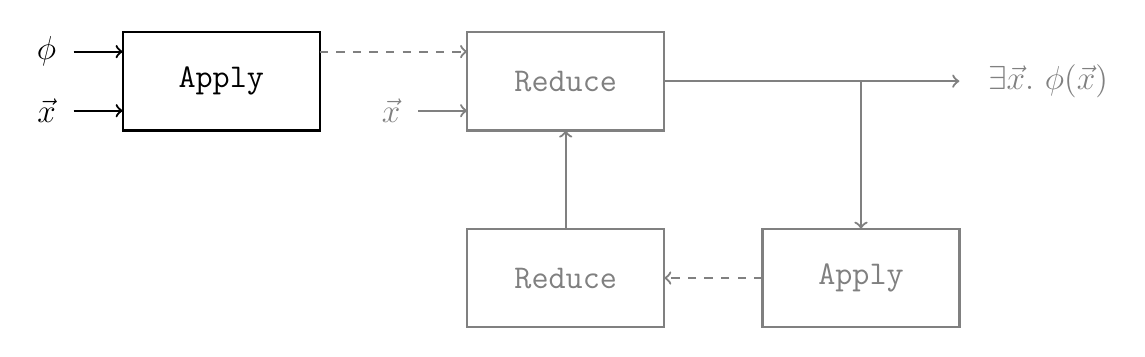
\begin{tikzpicture}[scale=1.25]
      % Boxes (outer)
      \draw[thick] (0,0) rectangle ++(2,1)
      node[pos=.5]{\large \texttt{Apply}};
      \draw[thick, gray] (3.5,0) rectangle ++(2,1)
      node[pos=.5]{\large \texttt{Reduce}};

      % Arcs (outer)
      \draw[->, thick] (-0.5,0.8) -- ++(0.5,0)
      node[pos=-0.55]{\large $\phi$};

      \draw[->, thick] (-0.5,0.2) -- ++(0.5,0)
      node[pos=-0.55]{\large $\vec{x}$};

      \draw[->, thick, dashed, gray] (2,0.8) -- ++(1.5,0);

      \draw[->, thick, gray] (3.0,0.2) -- ++(0.5,0)
      node[pos=-0.55]{\large $\vec{x}$};

      \draw[->, thick, gray] (5.5,0.5) -- ++(3,0)
      node[pos=1.3]{\large $\exists \vec{x}.\ \phi(\vec{x})$};

      % Boxes (inner)
      \draw[thick, gray] (6.5,-2) rectangle ++(2,1)
      node[pos=.5]{\large \texttt{Apply}};
      \draw[thick, gray] (3.5,-2) rectangle ++(2,1)
      node[pos=.5]{\large \texttt{Reduce}};

      % Arcs (inner)
      \draw[->, thick, gray] (7.5,0.5) -- ++(0,-1.5);

      \draw[->, thick, dashed, gray] (6.5,-1.5) -- ++(-1.0,0);

      \draw[->, thick, gray] (4.5,-1) -- ++(0,1);
    \end{tikzpicture}
  \end{figure}
\end{frame}

\begin{frame}
  \frametitle{Better Transposition: Deepest Variable Quantification}

  \begin{center}
    \LARGE

    $bdd\_exists(f, \max(\vec{x}))$
  \end{center}

  \bigskip

  \begin{block}{Motivation}
    Includes the first nested sweep inside of the transposition step.
  \end{block}

  \begin{block}{In Practice}
    Slows down computation time on average by $4.7\%$.
  \end{block}
\end{frame}

\begin{frame}
  \frametitle{Better Transposition: Pruning $\top$ Siblings}

  \begin{figure}
    \centering

    \begin{subfigure}{0.49\linewidth}
      \centering

      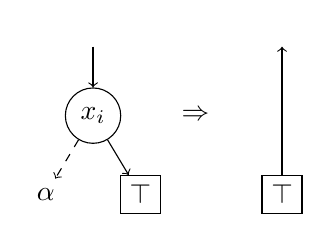
\begin{tikzpicture}
        % ------------------------------------------------------------------------
        % Before
        \node at (0, 1) (r) {};

        \node[shape = circle,    draw = black] at (0, 0) (n) {$x_i$};

        \node at (-0.6, -1) (alpha) {$\alpha$};
        \node[shape = rectangle, draw = black] at ( 0.6, -1) (T) {$\top$};

        \draw[->, dashed]
          (n) edge (alpha)
        ;
        \draw[->]
          (r) edge (n)
          (n) edge (T)
        ;

        \node at (1.3, 0) {$\Rightarrow$};

        % ------------------------------------------------------------------------
        % After
        \node at (2.4, 1) (r) {};

        \node[shape = rectangle, draw = black] at ( 2.4, -1) (T) {$\top$};

        \draw[<-]
          (r) edge (T)
        ;
      \end{tikzpicture}

      \caption{Pruning due to $\top$.}
    \end{subfigure}
    \begin{subfigure}{0.49\linewidth}
      \centering

      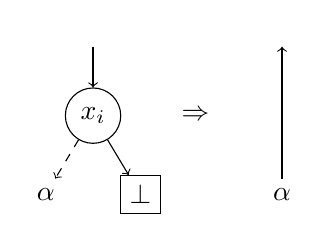
\begin{tikzpicture}
        % ------------------------------------------------------------------------
        % Before
        \node at (0, 1) (r) {};

        \node[shape = circle,    draw = black] at (0, 0) (n) {$x_i$};

        \node at (-0.6, -1) (alpha) {$\alpha$};
        \node[shape = rectangle, draw = black] at ( 0.6, -1) (F) {$\bot$};

        \draw[->, dashed]
          (n) edge (alpha)
        ;
        \draw[->]
          (r) edge (n)
          (n) edge (F)
        ;

        \node at (1.3, 0) {$\Rightarrow$};

        % ------------------------------------------------------------------------
        % After
        \node at (2.4, 1) (r) {};

        \node at ( 2.4, -1) (alpha) {$\alpha$};

        \draw[<-]
          (r) edge (alpha)
        ;
      \end{tikzpicture}

      \caption{Pruning due to $\bot$.}
    \end{subfigure}
  \end{figure}

  \begin{block}{In Practice}
    If it prunes subtrees, running time can improve up to $21\%$. Otherwise, it adds an overhead of
    up to $2\%$.
  \end{block}
\end{frame}

\begin{frame}
  \frametitle{Better Transposition: Partial Quantification}

  \begin{figure}
    \centering

    \begin{subfigure}{0.45\linewidth}
      \centering

      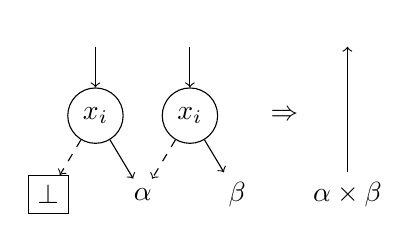
\begin{tikzpicture}
        % ------------------------------------------------------------------------
        % Before
        \node at (0, 1) (r) {};

        \node at (-0.6, 1) (r1) {};
        \node[shape = circle,    draw = black] at (-0.6, 0) (n1) {$x_i$};

        \node at ( 0.6, 1) (r2) {};
        \node[shape = circle,    draw = black] at ( 0.6, 0) (n2) {$x_i$};

        \node[shape = rectangle, draw = black] at (-1.2, -1) (F) {$\bot$};
        \node at ( 0.0, -1) (alpha) {$\alpha$};
        \node at (1.2, -1) (beta) {$\beta$};

        \draw[->, dashed]
          (n1) edge (F)
          (n2) edge (alpha)
        ;
        \draw[->]
          (r1) edge (n1)
          (n1) edge (alpha)
          (r2) edge (n2)
          (n2) edge (beta)
        ;

        \node at (1.8, 0) {$\Rightarrow$};

        % ------------------------------------------------------------------------
        % After
        \node at (2.6, 1) (r) {};

        \node at (2.6, -1) (prod) {$\alpha \times \beta$};

        \draw[<-]
          (r) edge (prod)
        ;
      \end{tikzpicture}

      \caption{Fully quantified pair of nodes.}
    \end{subfigure}
    \begin{subfigure}{0.54\linewidth}
      \centering

      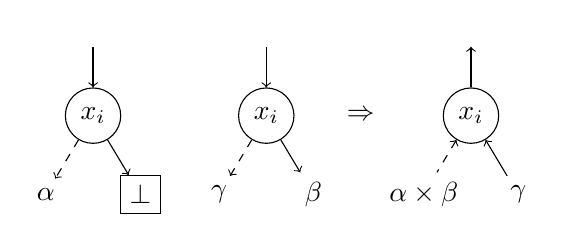
\begin{tikzpicture}
        \node at (0, 1) (r) {};

        \node at ( 0.0, 1) (r1) {};
        \node[shape = circle,    draw = black] at ( 0.0, 0) (n1) {$x_i$};

        \node at (-0.6, -1) (alpha) {$\alpha$};
        \node[shape = rectangle, draw = black] at ( 0.6, -1) (F) {$\bot$};

        \node at ( 2.2, 1) (r2) {};
        \node[shape = circle,    draw = black] at ( 2.2, 0) (n2) {$x_i$};

        \node at ( 1.6, -1) (gamma) {$\gamma$};
        \node at (2.8, -1) (beta) {$\beta$};

        \draw[->, dashed]
          (n1) edge (alpha)
          (n2) edge (gamma)
        ;
        \draw[->]
          (r1) edge (n1)
          (n1) edge (F)
          (r2) edge (n2)
          (n2) edge (beta)
        ;

        \node at (3.4, 0) {$\Rightarrow$};

        % ------------------------------------------------------------------------
        % After
        \node at ( 4.8, 1) (r) {};

        \node[shape = circle,    draw = black] at ( 4.8, 0) (nprod) {$x_i$};

        \node at ( 4.2, -1) (prod1) {$\alpha \times \beta$};
        \node at ( 5.4, -1) (prod2) {$\gamma$};

        \draw[<-, dashed]
          (nprod) edge (prod1)
        ;
        \draw[<-]
          (r) edge (nprod)
          (nprod) edge (prod2)
        ;
      \end{tikzpicture}

      \caption{Partially quantified pair of nodes.}
    \end{subfigure}
  \end{figure}

  \begin{block}{In Practice}
    In some instances, it improves performance by a factor of $\sim 2\times$.

    In others, it slows down by $\sim 2\times$.
  \end{block}

  \begin{block}{Observation}
    Instances improved by \emph{$\top$ Pruning} were disjoint from \emph{Partial Quantification}.
  \end{block}
\end{frame}

\blankframe

\begin{frame}
  \begin{table}
    \centering
    \begin{tabular}{l||ll|ll}
                                   & \multicolumn{2}{c|}{Single Quantification} & \multicolumn{2}{c}{Nested Sweeping}
      \\
                                   & LOC & \# Tests                              & LOC  & \# Tests
      \\ \hline \hline
      \texttt{nested\_sweeping.h}  & --  & --                                    & 1287 & 104
      \\
                                   &     &                                       &      &
      \\
      \texttt{quantify}            & 548 & 84                                    & 1152 & 152
      \\
      \quad \texttt{core/...}      & 326 & --                                    & 904  & --
      \\
      \quad \texttt{bdd/...}       & 122 & 64                                    & 157  & 108
      \\
      \quad \texttt{zdd/...}       & 100 & 20                                    & 20   & 44
    \end{tabular}
  \end{table}
\end{frame}

\blankframe

\begin{frame}
  \begin{figure}
    \centering

    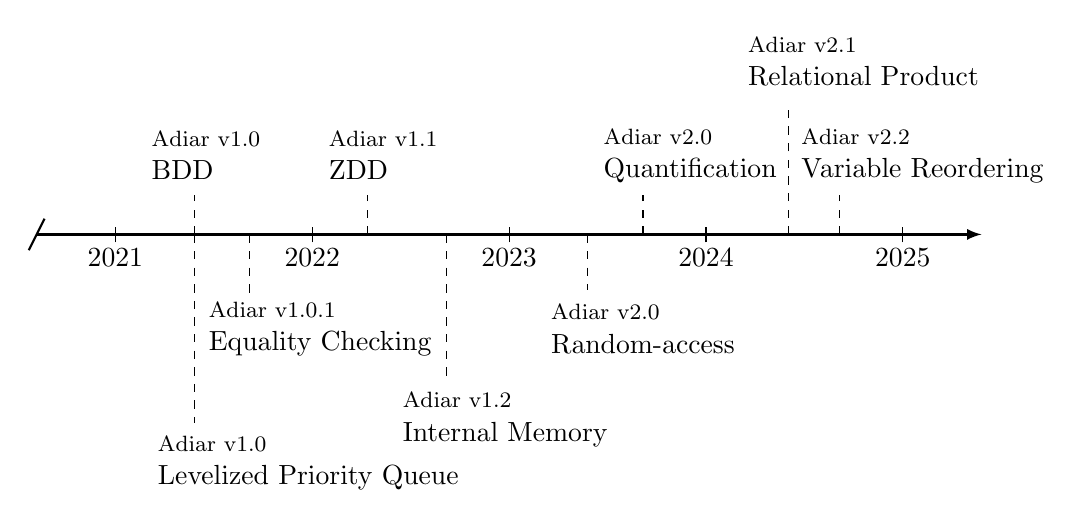
\begin{tikzpicture}
      % Primary line
\draw[-latex, thick] (0,0) -- (12,0);
\draw[thick] (0.1,0.2) -- (-0.1,-0.2);

% 2021
\draw (1,-0.1) -- ++(0,0.2);
\node at (1,-0.3) {$2021$};

\draw[dashed, color=black] (2,0) -- ++(0,0.5);
\node[color=black, align=left] at (2.15,1.0)
{\footnotesize Adiar v1.0\\BDD};

\draw[dashed, color=black] (2,0) -- ++(0,-2.4);
\node[color=black, align=left] at (3.45,-2.9)
{\footnotesize Adiar v1.0\\Levelized Priority Queue};

\draw[dashed, color=black] (2.7,0) -- ++(0,-0.8);
\node[color=black, align=left] at (3.6,-1.2)
{\footnotesize Adiar v1.0.1\\Equality Checking};

% 2022
\draw (3.5,-0.1) -- ++(0,0.2);
\node at (3.5,-0.3) {$2022$};

\draw[dashed, color=black] (4.2,0) -- ++(0,0.5);
\node[color=black, align=left] at (4.4,1.0)
{\footnotesize Adiar v1.1\\ZDD};

\draw[dashed, color=black] (5.2,0) -- ++(0,-1.8);
\node[color=black, align=left] at (5.95,-2.35)
{\footnotesize Adiar v1.2\\Internal Memory};

% 2023
\draw (6,-0.1) -- ++(0,0.2);
\node at (6,-0.3) {$2023$};

\draw[dashed, color=black] (7,0) -- ++(0,-0.7);
\node[color=black, align=left] at (7.7,-1.2)
{\footnotesize Adiar v2.0\\Random-access};

\draw[dashed, color=black] (7.7,0) -- ++(0,0.5);
\node[color=black, align=left] at (8.3,1.0)
{\footnotesize Adiar v2.0\\Quantification};

% 2024
\draw (8.5,-0.1) -- ++(0,0.2);
\node at (8.5,-0.3) (y2024) {$2024$};

\draw[dashed, color=black] (9.55,0) -- ++(0,1.6);
\node[color=black, align=left] at (10.5,2.2)
{\footnotesize Adiar v2.1\\Relational Product};

\draw[dashed, color=black] (10.2,0) -- ++(0,0.5);
\node[color=black, align=left] at (11.25,1.0)
{\footnotesize Adiar v2.2\\Variable Reordering};

% 2025
\draw (11,-0.1) -- ++(0,0.2);
\node at (11,-0.3) (y2025) {$2025$};
    \end{tikzpicture}
  \end{figure}
\end{frame}

\end{document}
